\documentclass[xcolor=dvipsnames,4pt,hyperref={colorlinks,citecolor=black,linkcolor=black,urlcolor=black}]{beamer}


\setbeamertemplate{navigation symbols}{}
\usefonttheme{professionalfonts}
\useinnertheme{circles}
\usepackage[spanish]{babel}
\usepackage[T1]{fontenc}
\usepackage[utf8]{inputenc}
\usepackage[orientation=portrait,size=custom,width=32,height=18]{beamerposter}

\usepackage{amsmath}
\usepackage{helvet}
%\usepackage[helvet]{sfmath}
\usepackage{eulervm}
\usepackage{units}
\usepackage{multirow}
\usepackage{graphicx}
\usepackage{tikz}
\usepackage{varwidth}

\usecolortheme[named=Black]{structure}

\usetikzlibrary{arrows,shapes,positioning,backgrounds,decorations.pathreplacing}

\PassOptionsToPackage{%
%backend=biber, % Instead of bibtex
backend=bibtex8,bibencoding=ascii,%
language=auto,%
%style=numeric-comp,%
style=authoryear-comp, % Author 1999, 2010
bibstyle=authoryear,dashed=false, % dashed: substitute rep. author with ---
sorting=ynt, % year, name, title
maxbibnames=3, % default: 3, et al.
backref=false,%
natbib=true, % natbib compatibility mode (\citep and \citet still work)
url=false, %
doi=false, %
eprint=false %
}{biblatex}
\usepackage{biblatex}

\addbibresource{library.bib}

\hypersetup{
% Uncomment the line below to remove all links (to references, figures, tables, etc), useful for b/w printouts
%draft,
colorlinks=true, linktocpage=true, pdfstartpage=3, pdfstartview=FitV,
% Uncomment the line below if you want to have black links (e.g. for printing black and white)
%colorlinks=false, linktocpage=false, pdfborder={0 0 0}, pdfstartpage=3, pdfstartview=FitV,
breaklinks=true, pdfpagemode=UseNone, pageanchor=true, pdfpagemode=UseOutlines,%
plainpages=false, bookmarksnumbered, bookmarksopen=true, bookmarksopenlevel=1,%
hypertexnames=true, pdfhighlight=/O,%nesting=true,%frenchlinks,%
urlcolor=webbrown, linkcolor=RoyalBlue, citecolor=Maroon, %pagecolor=RoyalBlue,%
%urlcolor=Black, linkcolor=Black, citecolor=Black, %pagecolor=Black,%
}

% My default font
%\usepackage{newcent}

% Computer Modern Bright font
%\usepackage{cmbright}

% Iwona light
%\usepackage[light,math]{iwona}

% LX fonts
%\usepackage{lxfonts}

% Malvern
%\input T1fmv.fd
%\renewcommand*\sfdefault{fmv}
%\renewcommand*\familydefault{\sfdefault}

% Comfortaa
%\usepackage[default]{comfortaa}

%\setbeamercolor{frametitle}{fg=NavyBlue}
%\setbeamercolor{structure}{fg=NavyBlue}
%\setbeamercolor{normal text}{fg=black}
\setbeamercolor{alerted text}{fg=NavyBlue}
%\setbeamercolor{example text}{fg=red}

\newcommand{\cl}[1]{\multicolumn{1}{c}{#1}}

\newenvironment{changemargin}[2]{%
  \begin{list}{}{%
    \setlength{\topsep}{0pt}%
    \setlength{\leftmargin}{#1}%
    \setlength{\rightmargin}{#2}%
    \setlength{\listparindent}{\parindent}%
    \setlength{\itemindent}{\parindent}%
    \setlength{\parsep}{\parskip}%
  }%
\item[]}{\end{list}}

\begin{document}
\tikzstyle{every picture}+= [remember picture]
\tikzstyle{every node} += [inner sep=1mm,font=\footnotesize]
\tikzstyle{nt} = [inner sep=2mm,font={\scshape\footnotesize}]
\tikzstyle{dr} = [draw=black!50,very thick]

\begin{frame}
\title{El ciclo de materia bariónica en las galaxias}
\author{Alfredo J. Mej\'ia}
\date{\today}

\maketitle
\end{frame}

%Motivación
\begin{frame}{\textsc{motivación}}
% Los estudios del contenido estelar en las galaxias distantes ($z\sim3$) solo tienen sentido en el
% límite de un número significativo de observaciones, pues debido a la gran variedad de fenómenos
% físicos que tienen lugar en estos sistemas (muchos aún en discusión) y distintas a las escalas
% temporales y espaciales en que estos ocurren, no es posible resolver las propiedades físicas de
% galaxias individuales de manera robusta. Por supuesto, las incertidumbres en los ingredientes de los
% modelos también juegan un papel importante. Aunque en principio en el universo local las galaxias se
% pueden resolver como imágenes extendidas en una exposición astronómica usando la técnica de la
% fotometría, la resolución espectral provista por esta clase de sondeos aunada al caracter degenerado
% del problema limitan considerablemente la información que se puede extraer de estos sondeos.

\begin{tikzpicture}[overlay]
% \draw[help lines] (0,-\textheight) grid (\textwidth,\textheight);

\node<-3> (hudf) at (7.5,-1) {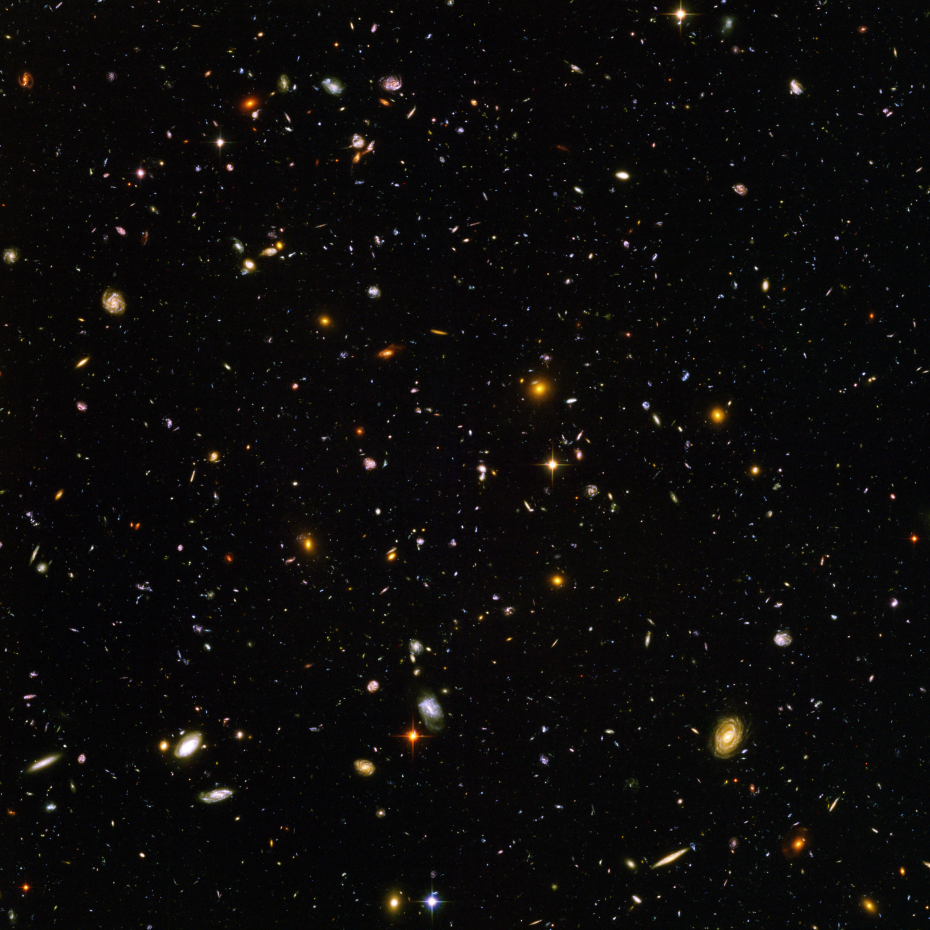
\includegraphics[height=15cm]{img/hudf}};
\node<2-3>[dr,circle,inner sep=2mm] (pag) at (7.5+4.08,0.79-1) {};
\node<3-3>[dr,circle,inner sep=2mm] (sfg) at (7.5+4.43,4.43-1) {};

\node<2-3> (pag-inset) at (20,-5) {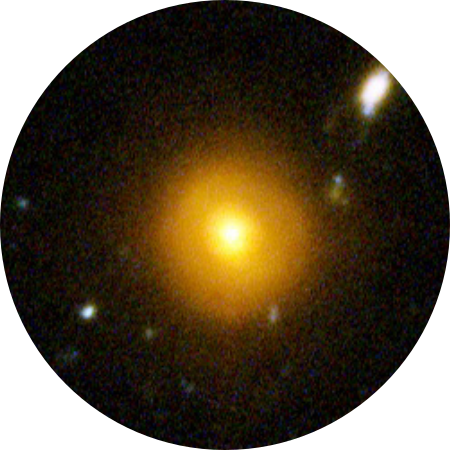
\includegraphics[width=0.2\textwidth]{img/hudf-pag-inset}};
\node<3-3> (sfg-inset) at (20,+3) {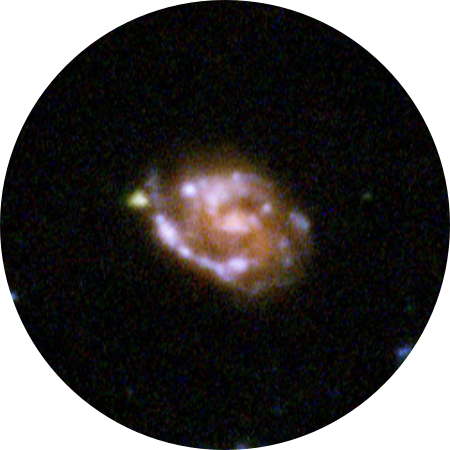
\includegraphics[width=0.2\textwidth]{img/hudf-sfg-inset}};
\path<2-3>[dr] (pag.east) -- (pag-inset.west);
\path<3-3>[dr] (sfg.east) -- (sfg-inset.west);

\node<2-5>[nt,right=of pag-inset] (pag-text) {galaxia temprana};
\node<3->[nt,right=of sfg-inset]  (sfg-text) {galaxia tardía};
\path<2-5>[-|,dr] (pag-inset.east) -- (pag-text.west);
\path<3-> [-|,dr] (sfg-inset.east) -- (sfg-text.west);

\node<4-5> (pag-mock) at (20,-5) {
\includegraphics[width=0.2\textwidth]{img/pag-mock}};
\node<4->  (sfg-mock) at (20,+3) {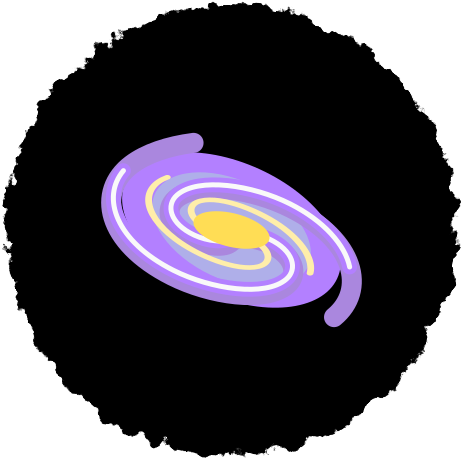
\includegraphics[width=0.2\textwidth]{img/sfg-mock}};

\node<5>[nt,left=2cm of pag-mock] (pag-desc) {
\begin{varwidth}{0.3\textwidth}
\begin{itemize}
\item[] dinámica estable
\item[] evolución pasiva
\item[] población vieja
\item[] MIE difuso
\end{itemize}
\end{varwidth}};
\node<5>[nt,left=2cm of sfg-mock] (sfg-desc) {
\begin{varwidth}{0.3\textwidth}
\begin{itemize}
\item[] dinámica inestable
\item[] formación estelar
\item[] población mixta
\item[] MIE multi-fase
\end{itemize}
\end{varwidth}};

\node<7->[left=2cm of sfg-mock]                           (sf-region) {
\includegraphics[width=0.2\textwidth]{img/sf-region}};
\node<7->[nt,left=of sf-region,text width=0.25\textwidth] (sf-region-text) {región de formación estelar};
\path<7->[dr]    (sfg-mock)       -- (sf-region);
\path<7->[-|,dr] (sf-region.west) -- (sf-region-text.east);

\node<8->[below=4cm of sf-region,label={[nt,name=molecule-label]90:moléculas}]      (molecule)    {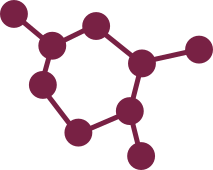
\includegraphics[scale=0.5]{img/molecule}};
\node<8->[left=1cm of molecule,label={[nt,name=dust-label]90:polvo}]                (dust)        {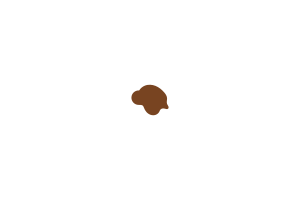
\includegraphics[scale=0.5]{img/dust}};
\node<8->[left=1cm of dust,label={[nt,name=stars-label]90:estrellas}]               (stars)       {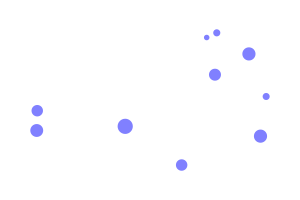
\includegraphics[scale=0.5]{img/stars}};
\node<8->[right=1cm of molecule,label={[nt,name=h-molecular-label]90:H\,i y H$_2$}] (h-molecular) {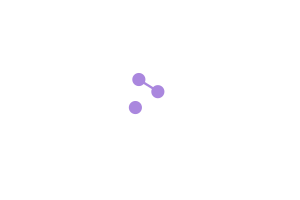
\includegraphics[scale=0.5]{img/h-molecular}};
\node<8->[right=1cm of h-molecular,label={[nt,name=ions-label]90:iones}]            (ions)        {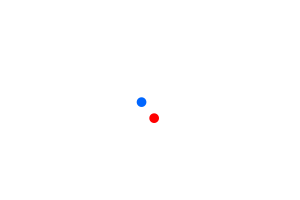
\includegraphics[scale=0.5]{img/ions}};
\path<8->[dr] (sf-region.south) -- (molecule-label.north);
\path<8->[dr] (sf-region.south) -- (dust-label.north);
\path<8->[dr] (sf-region.south) -- (stars-label.north);
\path<8->[dr] (sf-region.south) -- (h-molecular-label.north);
\path<8->[dr] (sf-region.south) -- (ions-label.north);

\node<9->[nt,above=3mm of sfg-mock]    {$\sim\unit[10]{kpc}$};
\node<9->[nt,above=3mm of sf-region]   {$\sim10\,$--$\,\unit[100]{kpc}$};
\node<9->[nt,below=3mm of stars]       {$\sim\unit[1]{UA}$};
\node<9->[nt,below=3mm of dust]        {$\sim\unit[1]{cm}$};
\node<9->[nt,below=3mm of h-molecular] {$\sim1\,$--$\,\unit[10]{\AA}$};
\draw<9->[decorate,decoration={brace,mirror,amplitude=2mm}] (molecule.south) -- (ions.south);

\end{tikzpicture}
\end{frame}

\begin{frame}{\textsc{motivación}}
\begin{tikzpicture}[overlay,node distance=5cm]
\tikzset{
  nr/.style={draw,very thick,inner sep=7mm,text width=3cm,text centered,font={\footnotesize\scshape\bfseries}},
  ar/.style={->,shorten >=1pt,draw,very thick},
  lb/.style={text width=2cm,text centered,font={\tiny\itshape}}
}
% \draw[help lines] (0,-\textheight) grid (\textwidth,\textheight);

\node[nr,circle] (cold-gas) at (0.5\textwidth,4cm) {gas frío};
\node[nr,circle,right=of cold-gas] (hot-gas)       {gas caliente};
\node[nr,circle,below=of cold-gas] (mig-gas)       {MIG};
\node[nr,circle,below right=of cold-gas] (stars)   {estrellas};

\path[ar] (cold-gas) edge [bend right=10] node[lb,above] {formación estelar} (stars);
\path[ar] (stars)    edge [bend right=10] node[lb,below] {reciclaje}         (cold-gas);
\path[ar] (hot-gas)  edge [bend right=10] node[lb,above] {enfriamiento}      (cold-gas);
\path[ar] (cold-gas) edge [bend right=10] node[lb,below] {re-calentamiento}  (hot-gas);
\path[ar] (cold-gas) edge                 node[lb,above] {eyección}          (mig-gas);
\path[ar] (mig-gas)  -|                   node[lb,left]  {re-incorporación}  (hot-gas);

\end{tikzpicture}
\end{frame}

\begin{frame}{\textsc{consideraciones teóricas}}

% Simplemente considerando el tiempo de vida de aquellas estrellas que contribuyen al enriquecimiento
% del medio interestelar, en el cual se formará la siguiente generación de estrellas, uno puede tener
% una idea de la escala típica de enriquecimiento químico en una galaxia.
\begin{columns}
\column{0.5\textwidth}
% Fig. 1 Yates+2013. Marcar los tiempos de AGB, de SNe Ia y SNe II
\begin{figure}
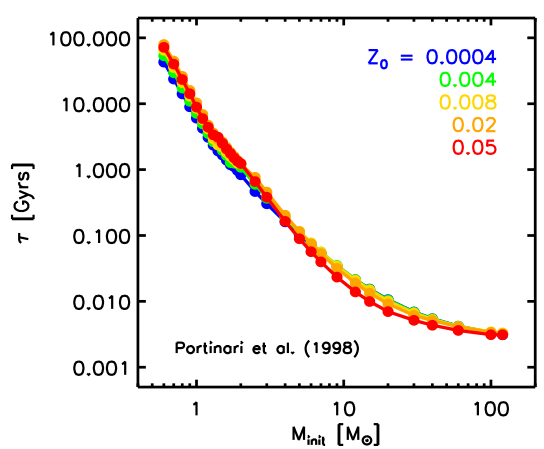
\includegraphics[scale=0.5]{img/yates2013-1}
\end{figure}
\column{0.5\textwidth}
%
% La masa eyectada por una población estelar entre $t_\text{ini}$ y $t_\text{fin}$ es
% \citep{Wiersma2009b}:
%
% $$ \Delta m_\star = m_{\star,0}\,\int_{m_\text{ini}}^{m_\text{fin}}\Phi(m)\,m_\text{e}(m,Z_0)\,\text{d}m $$
%
% donde $\int m\Phi(m)\,\text{d}m=1$.
\end{columns}
\end{frame}

\begin{frame}{\textsc{consideraciones teóricas}}

% Los vientos estelares de estrellas en fase AGB retornan especies
% Fig. 2 Yates+2013 (páneles inferiores).
\begin{figure}
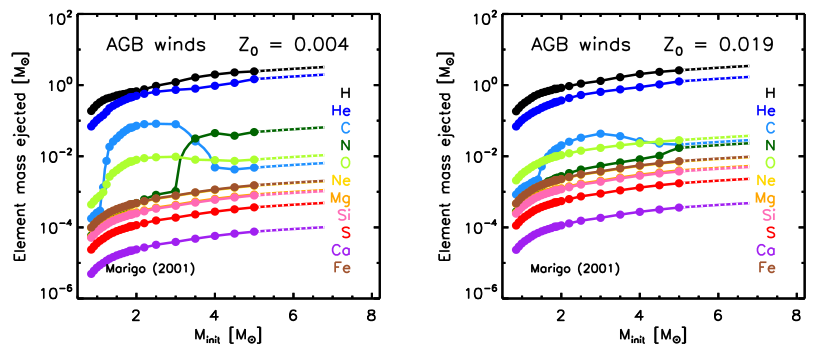
\includegraphics[scale=1]{img/yates2013-2}
\end{figure}
\end{frame}

\begin{frame}{\textsc{consideraciones teóricas}}

% Una supernova tipo II retorna especies químicas más pesadas que el O (e.\,g. Mg, Ca, Ti y Si) en
% cuestión de unos $10^7\,$años.
% Fig. 4 Yates+2013 (páneles inferiores). Mostrar líneas horizontales con la masa eyectada por SN Ia
\begin{figure}
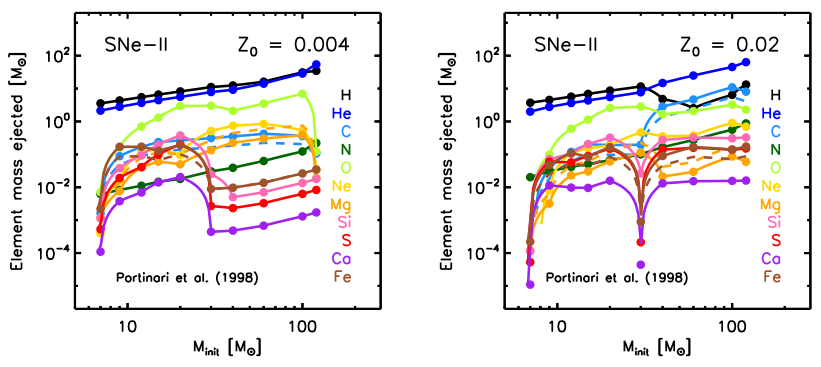
\includegraphics[scale=1]{img/yates2013-4}
\end{figure}
\end{frame}

\begin{frame}{\textsc{consideraciones teóricas}}

\begin{columns}
\column{0.5\textwidth}
% Fig. 3 Yates+2013.
\begin{figure}
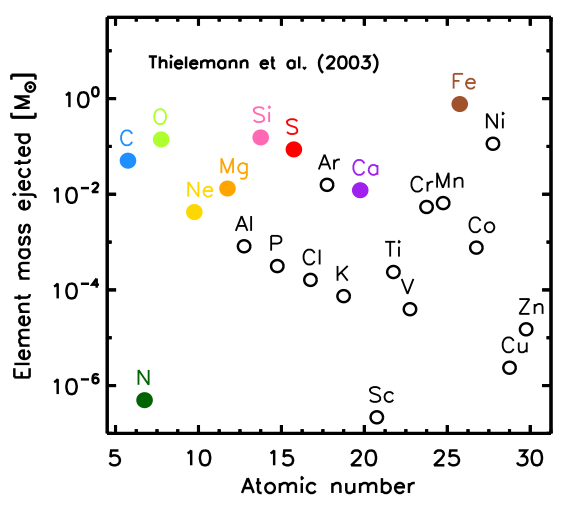
\includegraphics[scale=0.8]{img/yates2013-3}
\end{figure}
\column{0.4\textwidth}
Las supernovas tipo Ia enriquecen el medio con especies más pesadas que el Fe en una escala que
puede ir desde $10^7\,$años hasta $\sim10^9\,$años.
\end{columns}
\end{frame}

\begin{frame}{\textsc{consideraciones observacionales}}

En las estrellas de baja masa, que pueden vivir por $>3\times10^9\,$años muestran evidencia de esta
evolución química en sus distribuciones espectrales de energía \citep{Conroy2014}.
% Fig. 1 Conroy+2014. Resaltar rasgos usados por Worthey+1994 y Gallazzi+2005
\begin{figure}
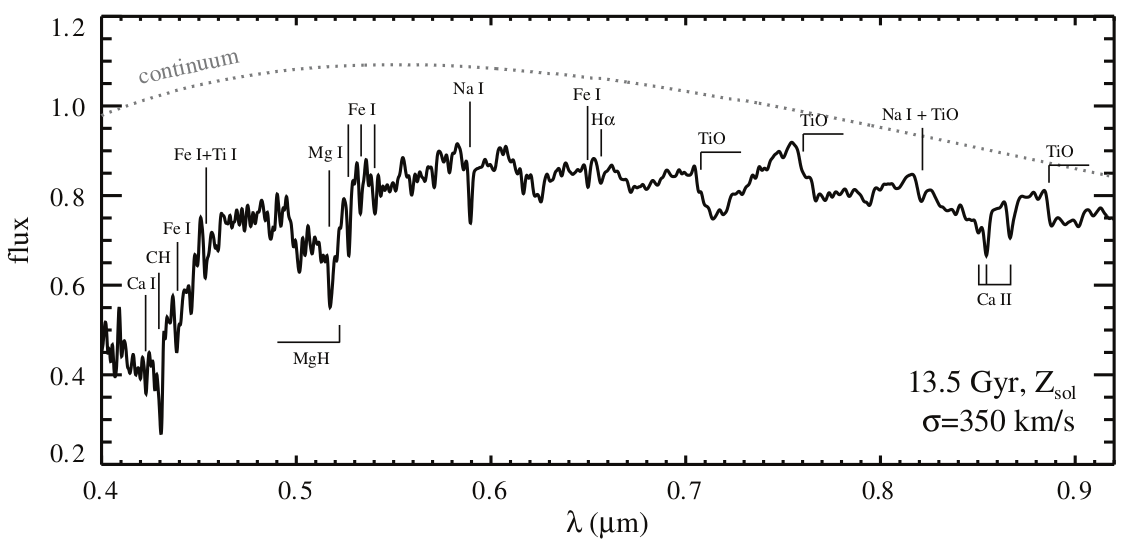
\includegraphics[scale=0.6]{img/conroy2014-1}
\end{figure}
\end{frame}
% En galaxias tempranas estas son las estrellas que dominan su distribución espectral de energía, por
% lo tanto no es sorprendente que la primera evidencia de una relación entre la edad y la metalicidad
% de una galaxia se encontrara en estos sistemas.

\begin{frame}{\textsc{consideraciones observacionales}}

% En galaxias tardías, los rasgos de metalicidad \emph{estelar} en el óptico son débiles, mientras que
% la emisión del MIE difuso permite estimar la metalicidad en fase de gas.
% Espectro del SDSS con sus líneas de emisión identificadas. Fig. 2 Calabro+2017
\begin{figure}
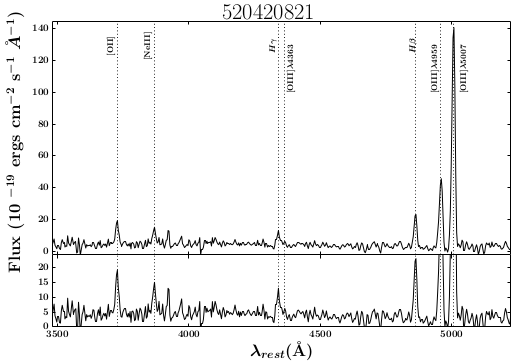
\includegraphics[scale=1]{img/calabro2017-2}
\end{figure}
% En estas galaxias es relativamente fácil estimar la TFE mediante la emisión de H$\alpha$, por
% ejemplo, de manera que se puede estudiar la primera relación fundamental del ciclo de masa
% bariónica.
\end{frame}

\begin{frame}{\textsc{relaciones clásicas --- $M_\star\,$--$\,\Psi$}}

\begin{columns}
\column{0.5\textwidth}
% La relación entre la masa y la tasa de formación estelar (TFE) es probablemente la relación más
% estudiada del ciclo de masa bariónica \citep[e.\,g.][]{Schmidt1959, Kennicutt1998}. Por ejemplo
% \citet{Brinchmann2004} estimó la TFE de las galaxias con formación estelar reciente del universo
% local muestreado por el SDSS. Ellos encuentran una correlación directa entre la masa estelar y la
% TFE.
\column{0.5\textwidth}
% Fig. 17 Brinchmann+2004. La dispersión a alta masa es probablemente debida a la dominancia de PaGs
\begin{figure}
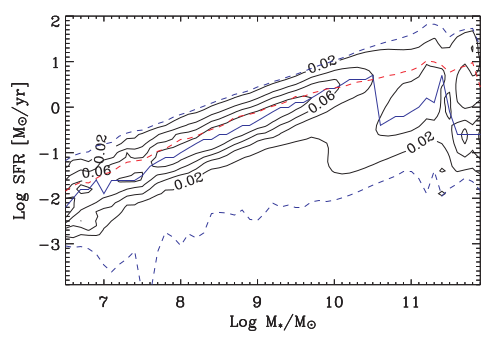
\includegraphics[scale=1]{img/brinchmann2004-17}
\end{figure}
\end{columns}
\end{frame}

\begin{frame}{\textsc{relaciones clásicas --- $M_\star\,$--$\,\Psi$}}
% Fig. 24 Brinchmann+2004
\begin{figure}
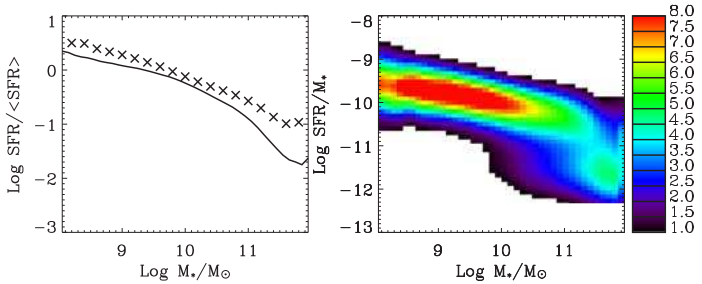
\includegraphics[scale=1]{img/brinchmann2004-24}
\end{figure}
\end{frame}

\begin{frame}{\textsc{relaciones clásicas --- $M_\star\,$--$\,\Psi$}}
% Ahora la masa por sí sola dice simplemente cuánto material bariónico existe en estrellas, pero no
% dice nada de como está distribuido el material que es, según la ley de Kennicutt-Schmidt, la
% relación fundamental entre la masa y la TFE. En este sentido, es interesante ver que la relación
% entre la TFE específica y la masa no es tan estrecha como la relación entre la TFE específica y la
% densidad superficial de masa. Un resultado que apunta a una relación con fenomenos del tipo local.
% Fig. 25 Brinchmann+2004
\begin{figure}
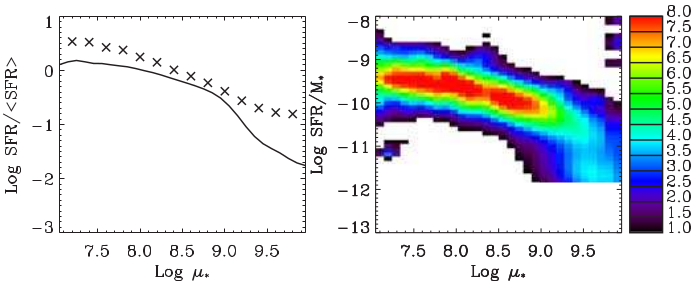
\includegraphics[scale=1]{img/brinchmann2004-25}
\end{figure}
\end{frame}

\begin{frame}{\textsc{relaciones clásicas --- $M_\star\,$--$\,\Psi$}}

\begin{figure}
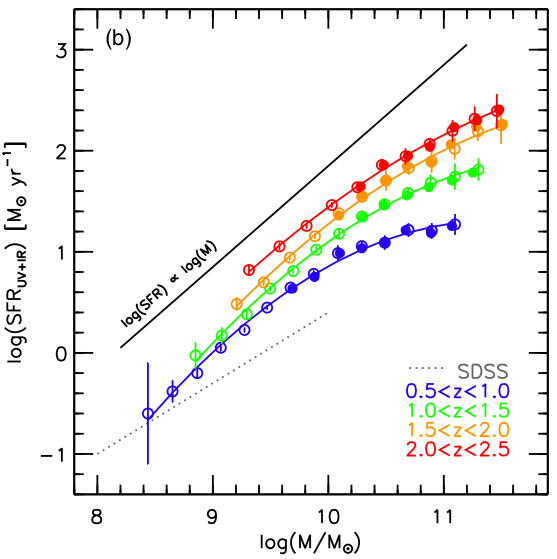
\includegraphics[scale=1]{img/whitaker2014-1}
\end{figure}
\end{frame}

\begin{frame}{\textsc{relaciones clásicas --- $M_\star\,$--$\,\Psi$}}

\begin{figure}
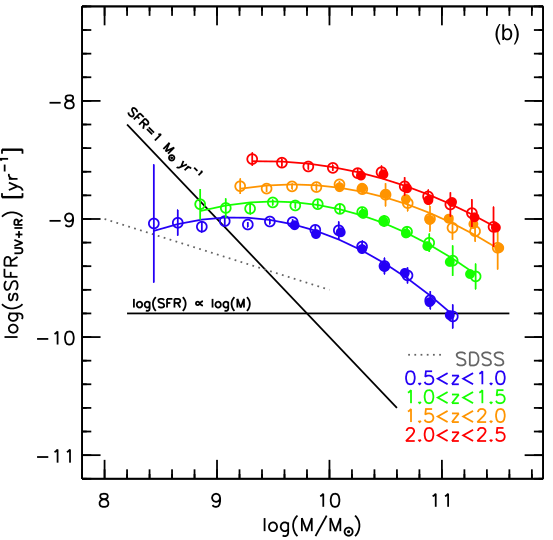
\includegraphics[scale=1]{img/whitaker2014-2}
\end{figure}
\end{frame}

\begin{frame}{\textsc{relaciones clásicas --- $t_\star\,$--$\,Z_\star$}}

% La relación entre la edad estelar y la metalicidad estelar no es trivial porque la formación estelar
% es un proceso cíclico: las estrellas nacen, enriquecen el MIE, mueren y luego otra generación de
% estrellas nace.
% mostrar diagrama explicando este ciclo en un esquema y en los planos edad--metalicidad--color
\begin{figure}

\includegraphics[scale=1]{img/placeholder}
\end{figure}
% En principio no se espera que haya una correlación entre ambas propiedades si no es
% por la degeneración entre ambas propiedades físicas. Sin embargo, considerando que la edad estimada
% es un momento de la HFE de la población estelar \citep{ocvirk2006a},
%
$$\Lambda(t) = \frac{\Psi(t)}{\Delta\lambda}\,\int_{\lambda_\text{min}}^{\lambda_\text{max}}\,L_\lambda^\text{PES}(Z;t)\,\text{d}\lambda$$
%
% se puede intuir que una correlación existe entre ambas propiedades físicas en una galaxia, pero esta
% probablemente no sería una correlación fundamental como la que se espera entre la metalicidad y la
% TFE.
\end{frame}

\begin{frame}{\textsc{relaciones clásicas --- $t_\star\,$--$\,Z_\star$}}
% En efecto, la relación entre la edad y la metalicidad se ha estudiado de manera extensiva en la
% literatura reciente. Fue primero observada en galaxias tempranas, aunque la degeneración entre la
% ambas propiedades físicas, dificulta la interpretación de esta relación \citep{Worthey1994}. La
% mayor parte de los estudios posteriores se concentró en sistemas tempranos, incluyendo bulbos de
% galaxias tardías \citep{Proctor2002, Terlevich2002}, probablemente debido a que ambos, los modelos
% de síntesis de poblaciones y los índices espectrales usados para estimar la edad y la metalicidad,
% favorecían particularmente el estudio de estos sistemas.
%
% Sin embargo, poco después \citet{Gallazzi2005} presentó un análisis de la relación edad-metalicidad
% que incluía galaxias tardías. Sus resultados se pueden resumir como sigue: ambos, la edad y la
% metalicidad están correlacionados con la masa estelar, aunque la fuerza de dicha correlación depende
% fuertemente del rango de masa. En general, las galaxias menos masivas están dominadas por
% poblaciones más jóvenes y menos ricas en metales pero con una dispersión estadística más grande,
% mientras que las más masivas están dominadas por poblaciones más viejas y más ricas en metales con
% dispersión estadística menor, esto último en acuerdo con los estudios previos de galaxias tempranas.
% Gráfico de la Tabla 2 Gallazzi+2005.
\begin{figure}

\includegraphics[scale=1]{img/placeholder}
\end{figure}
\end{frame}

\begin{frame}{\textsc{relaciones clásicas --- $t_\star\,$--$\,Z_\star$}}

% En el caso de las galaxias más masivas, la relación edad-metalicidad sugiere que estas se forman en
% escalas de tiempo más cortas ($\sim1\,$Gaño) que sus homólogas menos masivas.
% Fig. 12 Gallazzi+2005
\begin{figure}
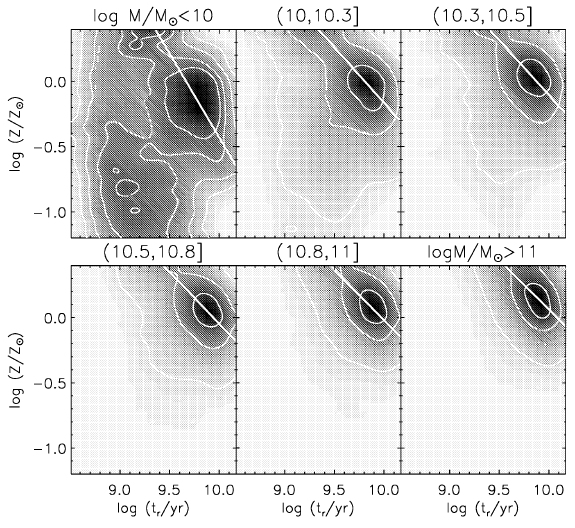
\includegraphics[scale=1]{img/gallazzi2005-12}
\end{figure}
\end{frame}

\begin{frame}{\textsc{relaciones clásicas --- $t_\star\,$--$\,Z_\star$}}

% Las galaxias menos masivas, por otro lado, se distribuyen en el plano edad-metalicidad dependiendo
% del tipo: dominadas por disco o dominadas por esferoides. Esto evidencia que la HFE presente podría
% depender de parámetros estructurales y/o fenómenos locales en estos sistemas.
% Fig. 11 Gallazzi+2005
\begin{figure}
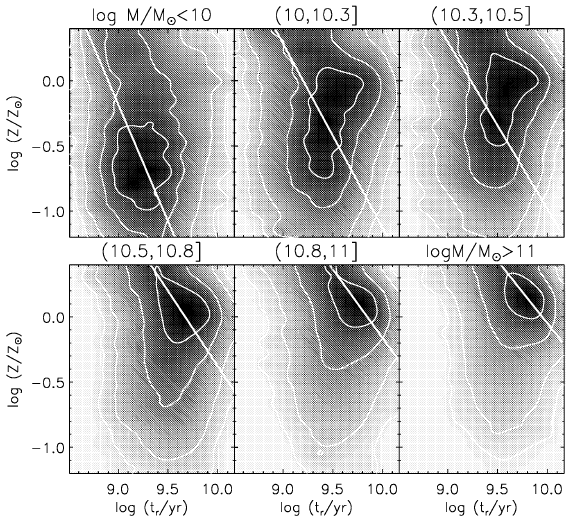
\includegraphics[scale=1]{img/gallazzi2005-11}
\end{figure}
\end{frame}

\begin{frame}{\textsc{relaciones clásicas --- $t_\star\,$--$\,Z_\star$}}

% Es importante notar, sin embargo, para las galaxias con formación estelar reciente, determinar la
% metalicidad es particularmente complicado, pues los trazadores de metalicidad en poblaciones jóvenes
% suelen ser débiles en el rango óptico debido al efecto del \emph{outshining}
% \citep[e.\,g.,][]{Conroy2013a}.
% Graficar la diferencia de espectros de 10Gaños para distintas Zs y una banda que represente la SNR típica.
\begin{figure}

\includegraphics[scale=1]{img/placeholder}
\end{figure}
\end{frame}

\begin{frame}{\textsc{relaciones clásicas --- $M_\star\,$--$\,Z$}}

% En los sistemas con formación estelar reciente, es particularmente sencillo estimar la metalicidad
% del MIE en fase de gas debido a la presencia de la emisión del gas. mostrar diagrama explicando la
% ionización del gas en el MIE
\begin{figure}

\includegraphics[scale=1]{img/placeholder}
\end{figure}
\end{frame}

\begin{frame}{\textsc{relaciones clásicas --- $M_\star\,$--$\,Z$}}

% \citet{Tremonti2004} estimaron la relación masa-metalicidad en una muestra de galaxias con formación
% estelar, usando como trazador de la metalicidad la abundancia de oxigeno. Encontraron una estrecha
% relación entre la metalicidad y la masa estelar, donde las galaxias menos masivas eran también menos
% ricas en metales, mientras que las más masivas eran más ricas en metales, un resultado en acuerdo
% con estudios previos.
% Fig. 6 Tremonti+2004
\begin{figure}
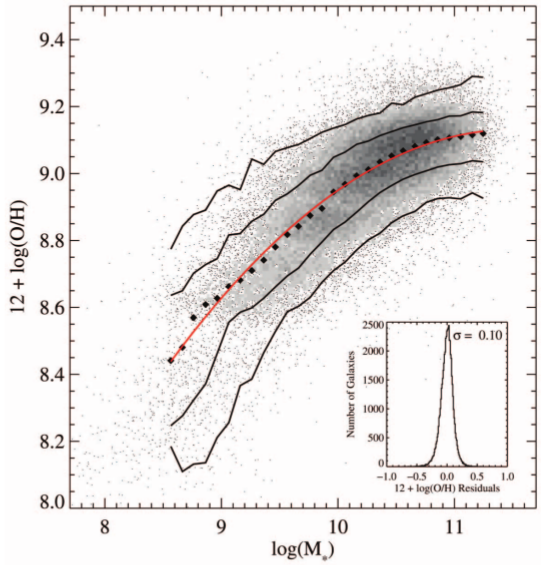
\includegraphics[scale=1]{img/tremonti2004-6}
\end{figure}
\end{frame}

\begin{frame}{\textsc{relaciones clásicas --- $M_\star\,$--$\,Z$}}

% \citeauthor{Tremonti2004} discutió dos hipótesis para explicar el origen físico de la relación
% masa-metalicidad. Si es que las galaxias más masivas forman una fracción de estrellas mayor que sus
% contrapartes menos masivas en un tiempo de Hubble, entonces la relación indica una secuencia de
% astración, i.\,e. las galaxias más masivas forman más estrellas que enriquecen el medio rápidamente,
% mientras que las galaxias menos masivas forman menos estrellas masivas de manera que los metales son
% encapsulados por más tiempo en las estrellas.
% Diagrama de región de formación estelar cada vez más eficiente formando metales como función de la masa estelar
\begin{figure}

\includegraphics[scale=1]{img/placeholder}
\end{figure}
\end{frame}

\begin{frame}{\textsc{relaciones clásicas --- $M_\star\,$--$\,Z$}}

% Si es que la eficiencia de la tasa de formación estelar es irrespectiva de la masa estelar, entonces
% las galaxias menos masivas de alguna forma han perdido de manera selectiva los metales, tal vez
% mediante vientos galácticos.
% Diagrama de galaxias en la secuencia de Hubble cada vez más eficientes perdiendo sus metales
\begin{figure}

\includegraphics[scale=1]{img/placeholder}
\end{figure}
\end{frame}

\begin{frame}{\textsc{relaciones clásicas --- $M_\star\,$--$\,Z$}}

% Evidencia de que la fracción másica de gas decrece con la masa estelar existe \citep{Bell2000} y
% podría explicar la relación masa-metalicidad en términos de que las galaxias menos masivas son menos
% eficientes formando estrellas masivas. Por otra parte, existe evidencia también de que las galaxias
% \emph{star-burst} sufren de fuertes vientos galácticos, que el medio intracúmulo y el medio
% intergaláctico están está enriquecidos en metales.

% De acuerdo con las expectativas de un modelo de caja cerrada, la metalicidad está directamente
% relacionada con el \emph{yield} estelar de la siguiente manera:
%
$$Z = y\ln{\left[{\mu_\text{gas}}^{-1}\right]},$$
%
% donde $y$ es el \emph{yield} y $\mu_\text{gas}$ es la fracción de masa en gas. Suponiendo que $y$ es
% constante (i.\,e. la TFE decrece continuamente en el tiempo). Dada una fracción de metales $Z$ y una
% fracción de masa en gas $\mu_\text{gas}$, usando esta relación se puede calcular el \emph{yield
% efectivo}, i.\,e. el \emph{yield} producido por las extrellas para observar \emph{al menos} la
% metalicidad $Z$. Si el modelo de caja cerrada efectivamente describe a las galaxias tardías como las
% de la muestra de \citeauthor{Tremonti2004}, entonces $y_\text{efectivo}=y$ independientemente de la
% masa bariónica. Sin embargo, lo que se observa es que $y_\text{efectivo}$ decrece con la masa
% bariónica.
% Fig. 8 Tremonti+2004
\begin{figure}
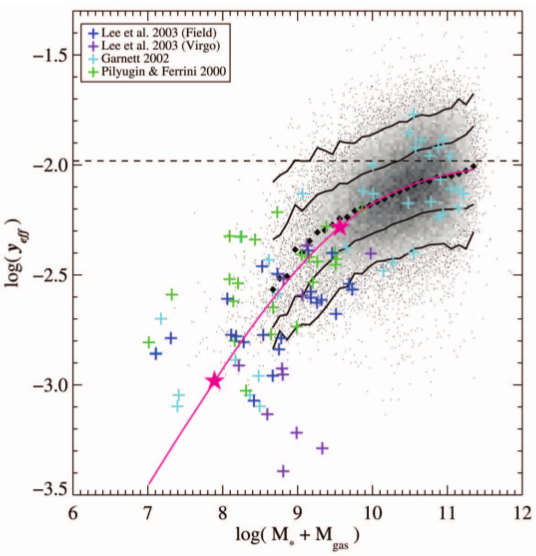
\includegraphics[scale=1]{img/tremonti2004-8}
\end{figure}
\end{frame}

\begin{frame}{\textsc{relaciones clásicas --- $M_\star\,$--$\,Z$}}
% Este hallazgo se interpreta como que la relación masa-metalicidad tiene un origen no solo en el
% fenómeno de formación estelar y en la subsiguiente evolución química, sino también en fenómenos
% reguladores en el MIE. Tal vez la evidencia más clara de que esto es así se puede apreciar en la
% relación entre la metalicidad estelar y la metalicidad del gas en el MIE:
% Fig. 9 Gallazzi+2005:
\begin{figure}
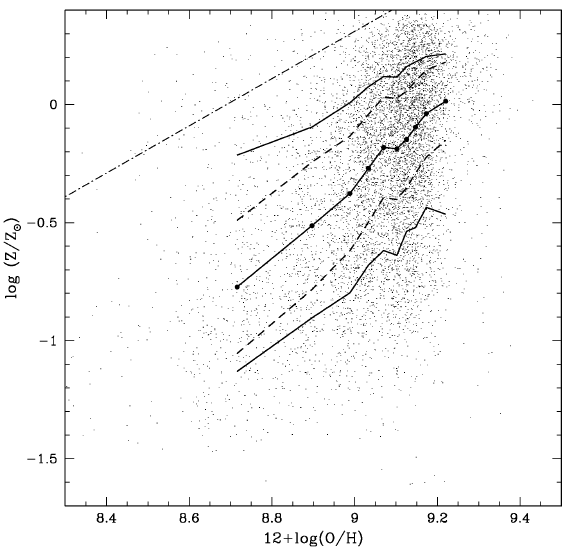
\includegraphics[scale=1]{img/gallazzi2005-9}
\end{figure}
% La metalicidad estelar es sistemáticamente menor que la metalicidad del gas en el MIE.
% Esto es evidencia clara de que los fenómenos reguladores están jugando un papel:
% - Enfriamiento del gas.
% - El feedback estelar.
% - Acreción de gas pristino del MIG.
% Además todos estos fenómenos están probablemente relacionados entre sí de una forma que no sabemos.
% El hecho de que se ha observado que el medio intergaláctico está enriquecido y que las galaxias
% \emph{star-burst} sufren fuertes vientos galácticos que superan la velocidad de escape, soportan
% esta hipótesis para explicar esta relación entre la masa y la metalicidad.

\end{frame}

\begin{frame}{\textsc{relaciones clásicas --- resumen}}
% describir de manera resumida los hallazgos importantes usando espectroscopía tradicional
\end{frame}

\begin{frame}{\textsc{relaciones clásicas --- resumen}}{\textbf{Incertidumbres observacionales.}}

% Algunos aspectos de estas dos escalas quedaban sin explicarse completamente y/o estaban plagadas de
% incertidumbres que limitaban una clara interpretación. Las fuentes de incertidumbres más importantes
% eran:

% Probablemente el efecto sistemático más importante en estos estudios es el efecto de apertura. Es
% bien sabido que existen gradientes radiales en las propiedades de las galaxias, por lo tanto,
% estudiar las relaciones entre las propiedades físicas `integradas', supone aproximaciones que deben
% tomarse en cuenta durante la interpretación de dichas relaciones.
% Fig. 1 Iglesias-Paramo+2013
\begin{figure}
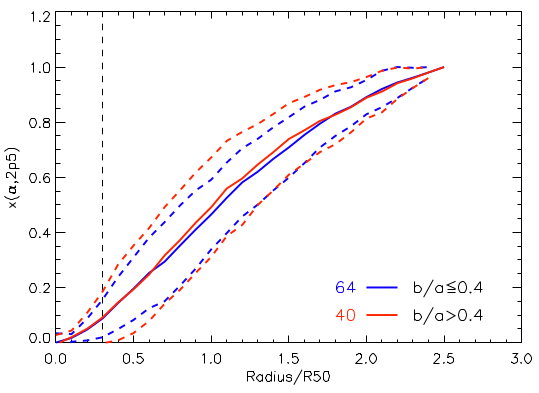
\includegraphics[scale=1]{img/iglesias-paramo2013-1}
\end{figure}
% Más cuidado aún se debe tener cuando se comparan propiedades integradas con diferentes aperturas. En
% este sentido las galaxias tempranas han ofrecido mejores posibilidades, pues exhiben gradientes
% menos en su contenido estelar como función de su radio. Las galaxias tardías por otro lado, no solo
% muestran gradientes más pronunciados en su contenido estelar, también tienen brillos superficiales
% típicamente menores y por lo tanto requieren tiempos de exposición más prolongados para alcanzar
% determinada $S/N$. Una alta $S/N$ es deseable en estos sistemas para determinar de manera confiable
% la metalicidad estelar usando rasgos espectrales como en \citet{Gallazzi2005}, generalmente más
% débiles que en galaxias tempranas. Resolución espacial es deseable para estudios de galaxias tardías
% para interpretar de manera adecuada las relaciones de escala, i.\,e. tomando en cuenta los efectos
% de gradientes radiales y de ángulo de inclinación.

\end{frame}

\begin{frame}{\textsc{relaciones clásicas --- resumen}}{\textbf{Incertidumbres en los modelos.}}

% Las galaxias tempranas de nuevo han sido favorecidas en el sentido de los modelos que usamos para
% interpretar su contenido estelar. Una población estelar simple por lo general es buena aproximación
% en estos sistemas, pues la relación masa luminosidad (en el óptico) evoluciona poco en poblaciones
% más viejas que unos pocos Gaños evolucionando pasivamente.
% mostrar evolución de M/L
\begin{figure}

\includegraphics[scale=1]{img/placeholder}
\end{figure}
% Las galaxias tardías, por otro lado suponen retos que dificultan la interpretación de sus
% propiedades integradas como ya vimos en el punto anterior. Adicionalmente modelos de HFE más
% complejos deben adoptarse para interpretar de manera adecuada su emisión en el espectro óptico,
% considerando otras componentes además de la estelar, como por ejemplo el contenido de polvo y de
% gas. Es costumbre estudiar estas componentes por separado, probablemente debido a la ausencia de
% modelos de poblaciones estelares que incluyan de manera consistente la emisión del gas, la
% absorción. El efecto del \emph{outshining} aunado al efecto de apertura atenta contra la
% interpretación de la masa estelar (usualmente menor que la masa real integrada de la galaxia) y de
% la metalicidad estelar. Varios intentos se han hecho por superar ambas limitaciones usando la
% resolución espacial provista por observaciones fotométricas \citep{Sorba2015} y sondeos en el
% cercano infrarrojo, donde el dicho efecto se espera sea menor \citep{Eminian2008}. Sin embargo, las
% incertidumbres en el modelado de la emisión de las estrellas en la fase TP-AGB en el cercano
% infrarrojo de nuevo dificultan la interpretación \citep{Zibetti2013}.

\end{frame}

\begin{frame}{\textsc{ciclo de masa visto por CALIFA}}
%
% La madurez alcanzada por los sondeos con IFU en la última década ha permitido la construcción de
% muestras de galaxias de todas las clases espectrales. La culminación del sondeo CALIFA
% \citep{Sanchez2012, Sanchez2016} ha significado un hito en este sentido, pues con el tercer
% \emph{public data release} se ha puesto a la disposición de la comunidad astronómica
% $\sim600\times1000$ espectros en el rango $\sim3000\,$---$\,7000\,$\AA{} para $\sim600$ galaxias en
% el universo local.
% Fig. 20 Husemann+2013.
\begin{figure}
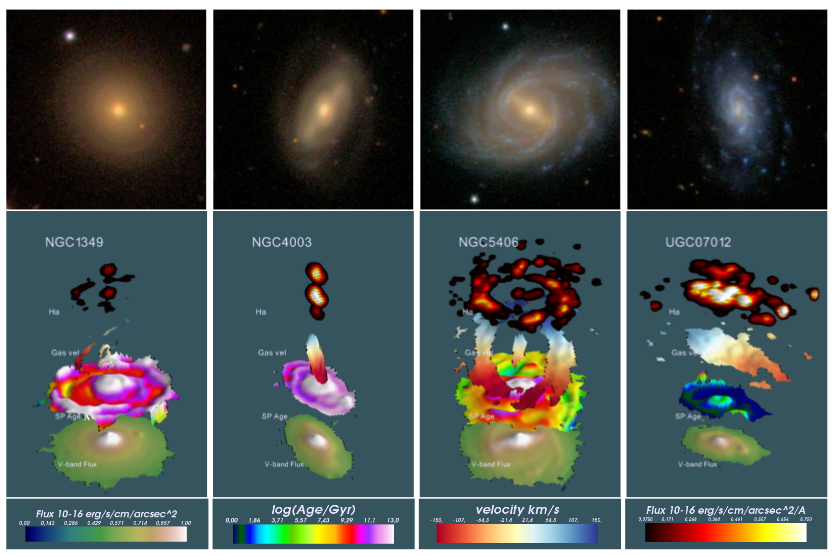
\includegraphics[scale=1]{img/husemann2013-20}
\end{figure}
% Ante las incertidumbres y las preguntas que quedaban abiertas respecto a la relación entre la edad,
% la masa y la metalicidad, sobre todo en sistemas con formación estelar, CALIFA presenta una
% oportunidad inigualable. Los estudios que buscaban desentrañar el caracter local de las relaciones
% de escala no tardaron en aparecer:
%
\end{frame}

\begin{frame}{\textsc{ciclo de masa visto por CALIFA --- $M\,$--$\,Z$}}

\citet{Rosales2012} estudia por primera vez la relación entre la masa, la metalicidad y la tasa de
TFE específica en $\sim2\,$k regiones H\textsc{ii} segregadas en una muestra de galaxias tardías
sondeadas por CALIFA.
% Fig. 1 Rosales-Ortega+2012:
\begin{figure}
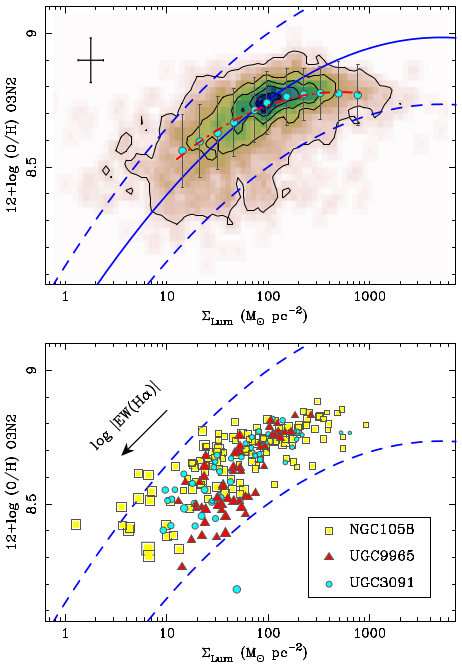
\includegraphics[scale=1]{img/rosales-ortega2012-1}
\end{figure}
\end{frame}

\begin{frame}{\textsc{ciclo de masa visto por CALIFA --- $M\,$--$\,Z$}}

% La similitud con la MMR global (Tremonti+2004) es sorprendente.
% Aún considerando unas pocas galaxias, el espacio de parámetros está bien muestreado.
% Pareciera haber una segunda correlación con el ancho equivalente de H$\alpha$.
% Esto sugiere que la MMR puede tener un origen local.
% Encontraron que la densidad superficial de masa y la metalicidad en las regiones H\textsc{ii} están
% directamente correlacionadas y ambas propiedades inversamente correlacionadas con la TFE específica.
% Fig. 3 Rosales-Ortega+2012. Intepretada como evidencia de downsizing local.
\begin{figure}
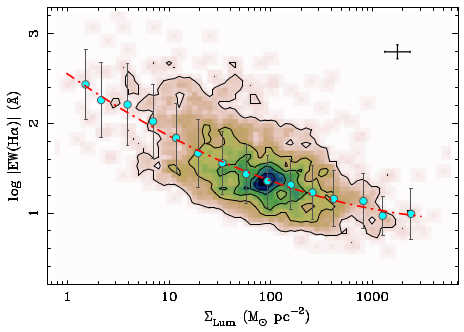
\includegraphics[scale=1]{img/rosales-ortega2012-3}
\end{figure}
% \citeauthor{Rosales2012} demostraron que la relación masa-metalicidad encontrada en estudios usando
% datos integrados (con efectos de apertura incluidos) puede explicarse como la suma de dos efectos:
% Dada la anticorrelación entre la TFE y la densidad superficial de masa.
% un crecimiento tipo \emph{inside-out}, en el que la región central de las galaxias se forma primero
% y luego la formación estelar se extiende sobre el disco; y un efecto de \emph{downsizing} local,
% donde las regiones más masivas forman estrellas más rápido y por lo tanto en una escala temporal más
% corta.
\end{frame}

\begin{frame}{\textsc{ciclo de masa visto por CALIFA --- $M\,$--$\,Z$}}

% Ambos fenómenos a su vez explican los gradientes radiales observados en galaxias con discos.
% Fig. 17 Gonzalez+2015:
\begin{figure}
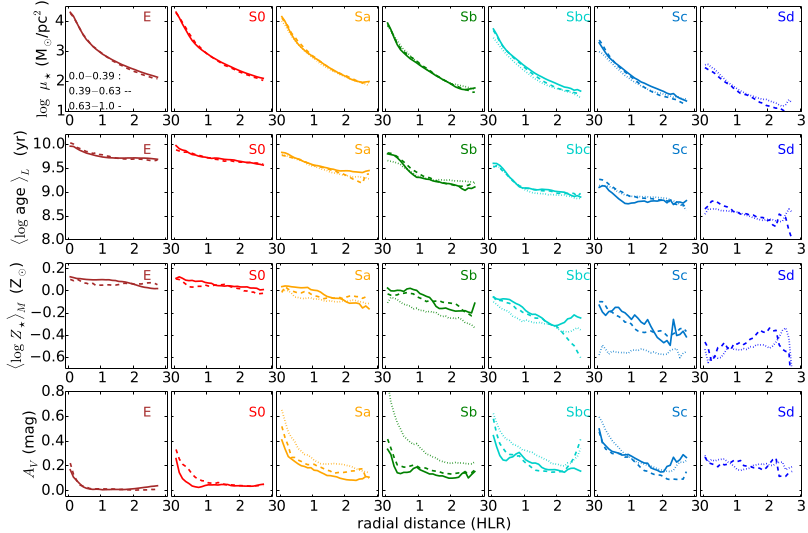
\includegraphics[scale=1]{img/gonzalez2015-17}
\end{figure}
% Los perfiles de densidad superficial de masa, de edad y de metalicidad decrecen con el radio
% Esto es consistente con los resultados de Rosales-Ortega+2012 y soportan el crecimiento inside-out.
% Es interesante notar también que el hecho de que la relación masa-metalicidad tenga un origen local
% sugiere que esta es en realidad una secuencia en astración, i.\,e., en las zonas de mayor formación
% estelar el enriquecimiento químico ocurre en una escala temporal más corta, mientras que en las de
% menor formación estelar los metales quedan atrapados en el interior de las estrellas de baja masa
% por más tiempo.
\end{frame}

\begin{frame}{\textsc{ciclo de masa visto por CALIFA --- $M\,$--$\,Z$}}

% Comparar el rol de los fenómenos locales y globales resulta entonces muy interesante de cara aun
% mejor entendimiento del ciclo de masa bariónica. \citet{Gonzalez2014b} estudió el rol de los efectos
% locales en la relación masa-metalicidad estelar. Ellos lograron recuperar las mismas tendencias en
% la relación masa-metalicidad (en fase de gas y estelar). Mostraron que la metalicidad en fase de
% gas, es trazador de la metalicidad en las poblaciones jóvenes, como es de esperarse en sistemas con
% formación estelar reciente donde el reciclaje ocurre en una escala de tiempo muy corta.
% Fig. 1 Gonzalez+2014b
\begin{figure}
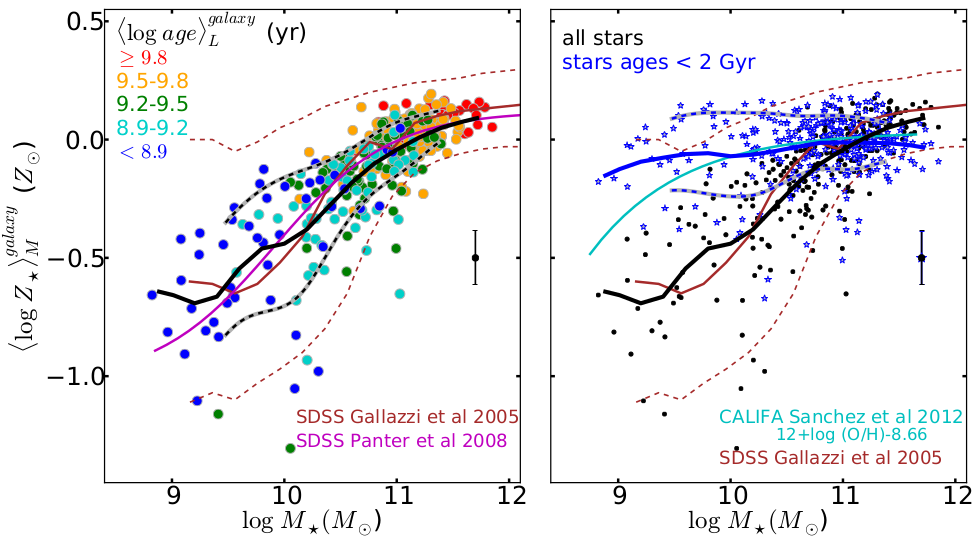
\includegraphics[scale=1]{img/gonzalez2014b-1}
\end{figure}
\end{frame}

\begin{frame}{\textsc{ciclo de masa visto por CALIFA --- $M\,$--$\,Z$}}

% La relación masa-metalicidad como función de la distancia al centro de las galaxias mostraba una
% dispersión en metalicidad que era claramente modulada por los efectos globales medidos por la masa
% estelar integrada de las galaxias. En las regiones menos densas (externas), por otro lado la
% densidad superficial de masa estelar correlaciona con la metalicidad estelar, como encontró
% \citet{Sanchez2013}. Más interesante aún, la relación masa-metalicidad depende del radio dentro de
% la galaxia donde, en acuerdo con los resultados en \citet{Gonzalez2014a}, la densidad de masa regula
% la metalicidad estelar, mientras que en las regiones más internas y por lo tanto más densas, la masa
% global regula la metalicidad.
% Fig. 3 Gonzalez+2014b
\begin{figure}
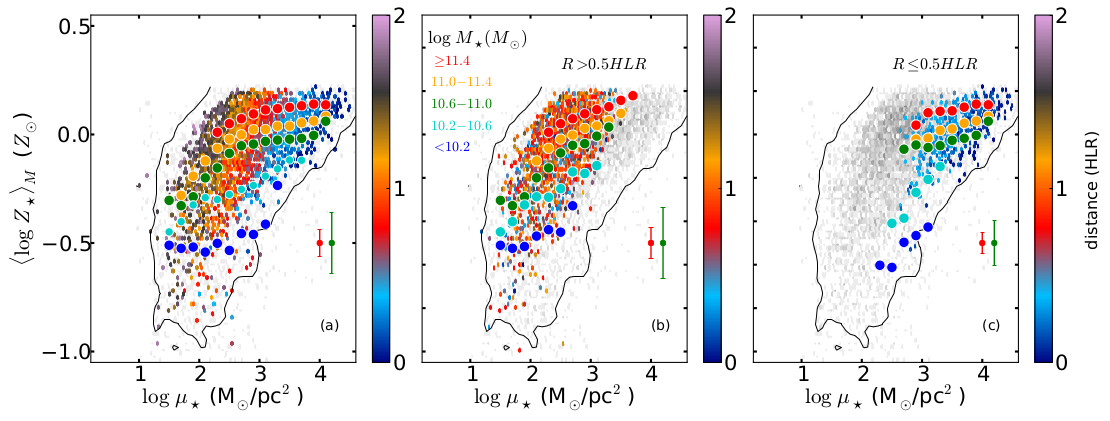
\includegraphics[scale=1]{img/gonzalez2014b-3}
\end{figure}
\end{frame}

\begin{frame}{\textsc{ciclo de masa visto por CALIFA --- $M\,$--$\,Z\,$--$\,\Psi$}}

% Esta relación, también llamada relación fundamental (o plano fundamental) de masa-metalicidad ya
% había sido estudiada \citep{Lara-Lopez2010, Mannucci2010} y tiene la siguiente forma: a una masa
% fija, las galaxias con mayor TFE tienen menor metalicidad y para galaxias de baja masa esta
% dependencia con la TFE es más fuerte. Existen varios fenómenos que pueden alterar la abundancia
% química presente en una galaxia: el enriquecimiento es producido en primer lugar por la formación y
% la evolución estelar, la acreción de material pristino del medio intergaláctico que diluye y
% disminuye la metalicidad, y las corrientes de salida que eyectan material enriquecido al medio
% intergaláctico.
% Fig. 1 Mannucci+2010.
\begin{figure}
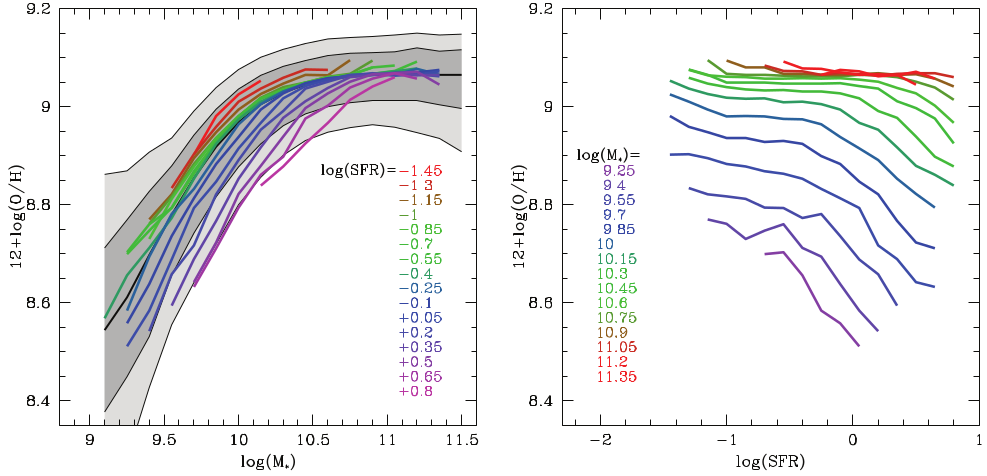
\includegraphics[scale=1]{img/mannucci2010-1}
\end{figure}
% La dispersión estadística en la relación masa-metalicidad se disminuye considerablemente si se introduce la TFE
% En galaxias menos masivas la dependencia entre la metalicidad y la TFE es fuerte
% En galaxias más masivas la dependencia es prácticamente inexistente
\end{frame}

\begin{frame}{\textsc{ciclo de masa visto por CALIFA --- $M\,$--$\,Z\,$--$\,\Psi$}}

% Sin embargo, \citet{Sanchez2013, Sanchez2017} mostró que la correlación entre la TFE y la
% metalicidad (local e integrada) es producto de ambos, el sesgo de apertura introducido por los
% sondeos espectroscópicos tradicionales y porque la relación entre la metalicidad y la TFE es
% inducida a través de la relación de estas dos propiedades con la masa estelar. Las relaciones
% masa-TFE y masa-metalicidad han sido conocidas desde hace mucho tiempo y a estas alturas ya no se
% discuten. La primera es entendida en el marco del fenómeno de acreción de gas del medio
% intergaláctico, mientras que la segunda es entendida en la capacidad de las galaxias por retener los
% metales que producen.
\begin{figure}
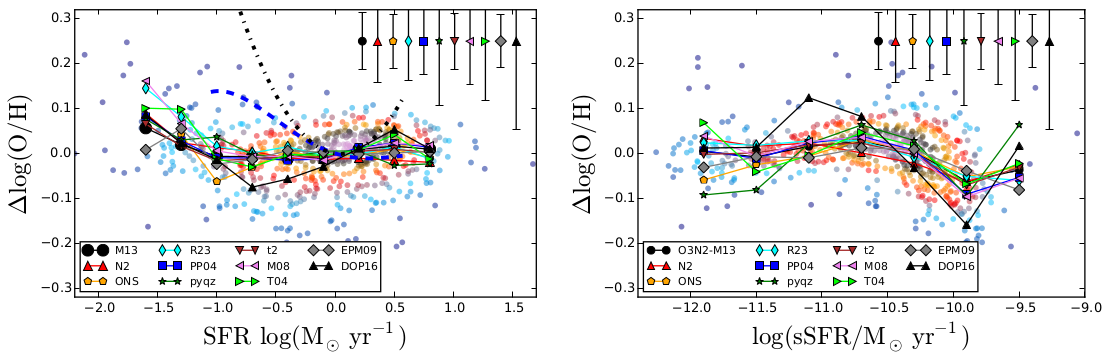
\includegraphics[scale=1]{img/sanchez2017-4}
\end{figure}
% Los resultados de \citeauthor{Sanchez2017} de nuevo ponen en el tapete la necesidad de introducir
% fenómenos reguladores para explicar de manera convincente la ausencia de una relación
% TFE-metalicidad.

\end{frame}

\begin{frame}{\textsc{ciclo de masa visto por CALIFA --- resumen}}
% resumir los hallazgos de CALIFA
\end{frame}

\begin{frame}{\textsc{una visión teórica del ciclo de masa --- caja cerrada}}

% mostrar una lista de los fenómenos
% mostrar esquema representando los reservorios de material bariónico
\begin{figure}
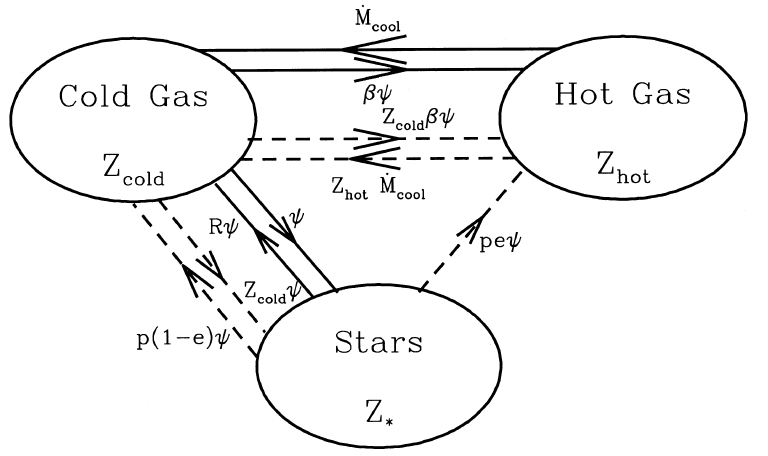
\includegraphics[scale=1]{img/cole2000-3}
\end{figure}

% Los fenómenos dinámicos son los más
% fundamentales, así que la masa estelar (como aproximación de la masa bariónica) y su densidad
% superficial serán consideradas cantidades importantes en el ciclo de masa. La masa sola contiene
% información global sobre la dinámica de la galaxia, mientras que la densidad superficial contiene
% información local.

% La capacidad del material bariónico en fase de gas para radiar su energía interna, define la escala
% temporal termodinámica en el que material del reservorio caliente se mueve al frío
% \citep{Wiersma2009b}.

% La formación estelar define la escala típica en que el material del reservorio frío se mueve al
% reservorio estelar \citep{Schaye2008}.
% Ecuación tau_* = M_* / TFE

\end{frame}

\begin{frame}{\textsc{una visión teórica del ciclo de masa --- caja cerrada}}

% Ahora, dos preguntas interesantes después de haber visto lo que las observaciones indican y en el
% marco de estos procesos físicos son: ¿en qué escala temporal ocurre el enriquecimiento químico? y
% más importante aún ¿por qué este parece ser independiente de la TFE? en el esquema anterior está
% representado esquemáticamente el ciclo de masa bariónica en una galaxia. Tres reservorios son
% importantes: el estelar y los de gas caliente y frío. Por supuesto entre los tres habrá intercambio
% de materia debido a los procesos de enfríamiento del gas caliente, la formación estelar y el
% \emph{feedback} debido a vientos estelares y explosiones de supernova. Dependiendo de las
% propiedades dinámicas de la galaxias, una fracción del material expulsado por las estrellas puede ir
% directo al reservorio de gas caliente.

% Debido a la evolución estelar, parte del material devuelto al MIE está enriquecido químicamente, de
% manera que las siguientes generaciones de estrellas tendrán una metalicidad cada vez más alta.
% Suponiendo conservación de la masa, el transporte de material de un reservorio a otro puede
% describirse mediante las ecuaciones de continuidad:
%
\begin{subequations}
\begin{align}
\dot{M}_\star         &= (1-R)\psi \\
\dot{M}_\text{hot}    &= -\dot{M}_\text{cool} + \beta\psi \\
\dot{M}_\text{cold}   &= \dot{M}_\text{cool} - (1-R+\beta)\psi \\
\dot{M}_\star^Z       &= (1-R)Z_\text{cold}\psi \\
\dot{M}_\text{hot}^Z  &= -\dot{M}_\text{cool}Z_\text{hot} + (pe+\beta Z_\text{cold})\psi \\
\dot{M}_\text{cold}^Z &= \dot{M}_\text{cool}Z_\text{hot} + [p(1-e)-(1+\beta-R)Z_\text{cold}]\psi
\end{align}
\end{subequations}
\end{frame}

\begin{frame}{\textsc{una visión teórica del ciclo de masa --- caja cerrada}}

% Ahora, estamos particularmente interesados en calcular la TEQ estelar y en fase de gas (frío),
% porque son las que podemos estimar a partir de las observaciones con relativa facilidad. Usando la
% relación $Z\equiv M^Z/M$ y las ecuaciones del ciclo de masa tenemos que:
%
\begin{subequations}
\begin{align}
\dot{Z}_\star       &= (1-R)\frac{\psi}{M_\star}(Z_\text{cold}-Z_\star) \\
\dot{Z}_\text{cold} &= (Z_\text{hot}-Z_\text{cold})\frac{\dot{M}_\text{cool}}{M_\text{cold}} + p(1-e)\frac{\psi}{M_\text{cold}}
\end{align}
\end{subequations}
\end{frame}

\begin{frame}{\textsc{una visión teórica del ciclo de masa --- caja cerrada}}

% Es interesante notar que el enriquecimiento químico estelar ocurre en la misma escala temporal en
% que ocurre la formación estelar
%
$$\tau_\text{TFE} = (4\pm1)\times\unit[10^9]{años}\left[\frac{\Sigma_\text{frio}}{\unit[1]{M_\odot\,pc^{-2}}}\right]$$
%
% De manera que las conclusiones de \citet{Gonzalez2014b} cobran
% sentido en el terreno teórico: el enriquecimiento químico estelar depende de ambos, fenómenos
% locales ($\mu_\star\sim\Sigma_\text{cold}$) que regulan la evolución química y globales ($M_\star$)
% que modulan la amplitud de esta.

% La TEQ del gas en el reservorio frío depende de la tasa de enfríamiento y de la TFE. Intuitivamente
% se espera que la escala temporal dinámica sea más corta que la escala térmica. Sin embargo, bajo
% ciertas circunstancias (densidad, temperatura y metalicidad) la escala temporal de enfriamiento
% puede ser más corta.
% Fig. 3b Wiersma+2009
\begin{figure}
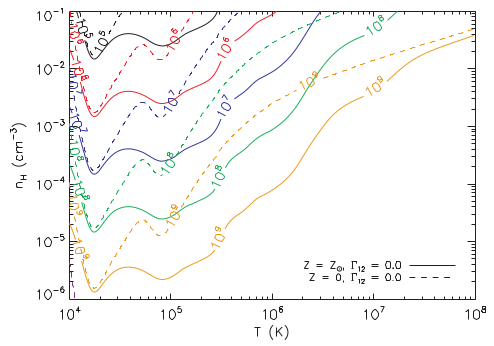
\includegraphics[scale=1]{img/wiersma2009-3}
\end{figure}
% De hecho la dependencia de la escala temporal de enfriamiento con la densidad, la temperatura y la
% metalicidad del gas caliente es:
%
$$\tau_\text{enf} \approx \unit[10\times10^9]{años}\left[\frac{T}{\unit[10^7]{K}}\right]%
\left[\frac{\unit[10^{-3}]{g\,cm^{-3}}}{\rho_\text{cal}}\right]\left[\frac{\unit[10^{-23}]{erg\,cm^3}}{\Lambda_n}\right]$$

\end{frame}

\begin{frame}{\textsc{una visión teórica del ciclo de masa --- caja cerrada}}

% Si comparamos ambas escalas temporales tenemos:
%
\begin{equation*}
\frac{\tau_\star}{\tau_\text{cool}} \approx 0.4\left(\frac{\Sigma_\text{cold}}{1\,\text{M}_\odot\,\text{pc}^{-2}}\right)^{-0.4}\left(\frac{10^7}{T_\text{hot}}\right)\left(\frac{\rho_\text{hot}}{10^{-3}\,\text{cm}^{-3}}\right)\left(\frac{\Lambda(T_\text{hot},Z_\text{hot})}{10^{-23}\,\text{erg\,cm}^{3}\,\text{s}^{-1}}\right)
\end{equation*}
%
\begin{figure}
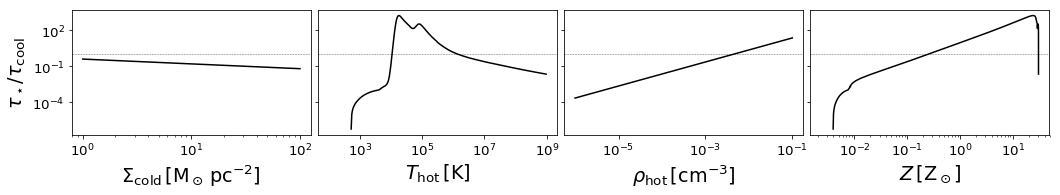
\includegraphics[scale=1]{img/time_scales}
\end{figure}
% En la figura se muestra el comportamiento de esta fracción variando los cuatro parámetros que
% interesan uno a la vez. Es claro que en la mayoría de los casos la escala temporal de formación
% estelar es más corta que la escala temporal de enfriamiento. La temperatura del reservorio caliente
% es el parámetro más sensible y que puede disminuir drásticamente la escala temporal de enfriamiento
% en el rango de plausibilidad. Es seguido por la metalicidad en el reservorio caliente y valores
% extremos de la densidad.

\end{frame}

\begin{frame}{\textsc{una visión teórica del ciclo de masa --- caja cerrada}}

% Las observaciones de que el gas está enriquecido en galaxias con formación estelar en un amplio
% rango de masa estelar ($10^{10}\,$---$\,10^{12}\,\text{M}_\odot$)
% Fig. 1 Gonzalez+2014
\begin{figure}
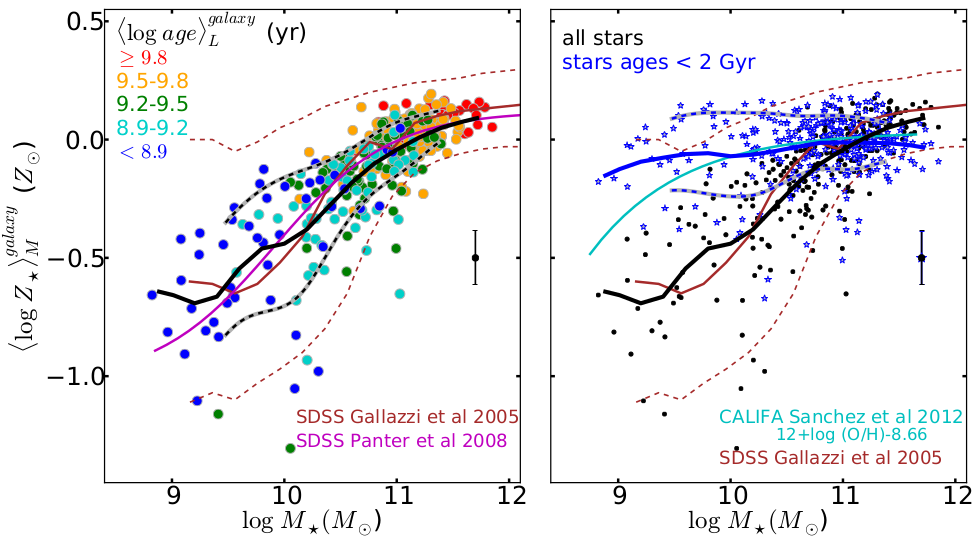
\includegraphics[scale=1]{img/gonzalez2014b-1}
\end{figure}
% mientras que las estrellas son comparativamente pobres en metales, respalda la hipótesis de que la
% formación estelar ocurre en una escala temporal larga en comparación con el enfriamiento de gas. Sin
% embargo resulta curioso que aunque en estas galaxias la formación estelar no es tan eficiente, el
% gas luzca tan enriquecido. Por ejemplo, una galaxia de $M_\star=10^{10}\,\text{M}_\odot$ forma una
% masa solar por año, mientras que galaxias más masivas pueden formar hasta diez masas solares por año
% \citep{Sanchez2013}. ¿Cómo llegó a enriquecerse el gas? Uno puede especular que estas galaxias
% sufrieron eventos de formación estelar importante en el pasado que pudo enriquecer el medio
% relativamente rápido, en cuyo caso ¿por qué la formación estelar ya no es tan eficiente ahora? Esta
% línea de razonamiento necesariamente conduce a que, aunque el enriquecimiento químico es catalizador
% para el enfríamiento del gas, no necesariamente promueve la formación de estrellas, especialmente de
% estrellas masivas capaces de enriquecer el MIE.

\end{frame}

\begin{frame}{\textsc{una visión teórica del ciclo de masa --- caja abierta}}

\begin{figure}
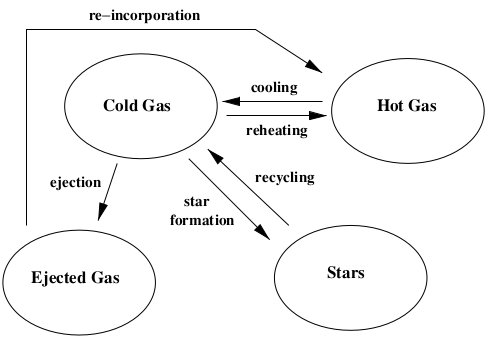
\includegraphics[scale=1]{img/delucia2004-1}
\end{figure}
% Uno puede irse por caminos más exóticos, especulando que estas galaxias obtienen el gas enriquecido
% del MIG y no por formación estelar. Lo cual está soportado por observaciones de gas enriquecido en
% el medio intracúmulo, sin embargo estas galaxias parecen haber formado sus estrellas pasivamente en
% una escala temporal que puede ser tan larga como la edad del universo. De manera que el
% enriquecimiento probablemente ha ocurrido \emph{in situ}.

% Durante la mayor parte de la discusión anterior se asumió
% implicitamente que las galaxias se comportan como cajas cerradas. Sin embargo el hecho de que el MIG
% se encuentre enriquecido en algunos casos definitivamente refuta esa hipótesis. La pregunta se
% reduce entonces a ¿es el fenómeno de \emph{feedback} suficiente para remover efectivamente material
% enriquecido del MIE?

% Intuitivamente uno espera que el enriquecimiento químico del MIG ocurra en una escala temporal más
% larga que la del enriquecimiento del MIE. Por lo tanto, el material acretado por los halos
% galácticos debe ser pobre en metales en comparación con el gas presente en el MIE. En este sentido,
% el material acretado actúa como un disolvente de la metalicidad en fase de gas, pero al mismo
% tiempo, de acuerdo con la discusión anterior, potencia la formación de estrellas contaminantes. En
% este escenario entonces, la tasa de enriquecimiento químico efectiva dependerá de la capacidad de
% las galaxias para retener el material enriquecido durante etapas de \emph{feedback} estelar
% importantes. De nuevo, esto ocurre en una escala dinámica, esta vez global, probablemente
% relacionada con la masa estelar total.

% Las galaxias de baja masa muestran una caída abrupta en la metalicidad en fase de gas en función de
% la masa, aún así esta es sistemáticamente mayor que la metalicidad estelar. Ya que para enriquecer
% el MIE, estas debieron haber formado estrellas contaminantes en algún momento, las cuales son además
% las únicas capaces de barrer material enriquecido fuera del halo, la única forma de que estas
% galaxias sean sistemáticamente pobres en metales es que nunca hayan formado este tipo de estrellas.
%
\end{frame}

\begin{frame}{\textsc{prólogo --- expectativas para el futuro}}
%
% Los procesos locales responsables de regular la formación estelar y el enriquecimiento químico, son
% probablemente los tópicos más relevantes en la literatura extragaláctica en la actualidad. Mucho se
% ha avanzado desde el punto de vista observacional con los sondeos de IFS. En este sentido, CALIFA ha
% marcado un hito, pues ha puesto a la disposición de la comunidad científica espectroscopía de campo
% integrado de una muestra de $\sim600$ galaxias distribuidas a lo largo de la clasificación de
% Hubble. Ahora podemos decir con seguridad que ambos, los efectos globales y los locales determinan
% la HFE en las galaxias y que el paradigma de caja cerrada comunmente adoptado para decir algo
% respecto al enriquecimiento químico, no tiene cabida de manera universal, no entre galaxias ni
% dentro de una misma galaxia. Quedan aún incertidumbres sobre el rol relativo que juegan la TFE, los
% vientos galácticos y el acrecimiento de material enriquecido presente en el medio intergaláctico. El
% \emph{feedback} estelar se ha invocado para explicar la ausencia de metales en el medio interestelar
% \citep{Tremonti2004, Kobayashi2007}. Las variaciones en la función inicial de masa se han invocado
% como un mecanismo adicional para explicar la ausencia de metales en las galaxias menos masivas
% \citep{Koppen2007}. Todos estos mecanismos se ha medido tanto en observaciones como en simulaciones
% en estudios independientes, mas aún no son mutuamente excluyentes. Determinar cual(es) y bajo que
% circunstancias actúan para regular la HFE en las galaxias, será tópico de investigación por los
% próximos años.
%
\end{frame}

% Apéndice =========================================================================================

%Historia
\begin{frame}[allowframebreaks]{\textsc{Antecedentes de sondeos con IFU}}
%
El problema de adquisición de imágenes astronómicas es, en el sentido general, un problema de dos
dimensiones espaciales y una dimensión espectral $(x,y;\lambda)$. Desafortunadamente, debido a
limitaciones de ingeniería, la mayoría de los esfuerzos que ofrecen una resolución espectral
$R\sim1000$, están limitados a una dimensión espacial, i.\,e. $(x;\lambda)$. El uso del formato
\emph{long-slit} (rendija) resuelve parcialmente el problema de la dimensión perdida por
espectrógrafos convencionales: si la dispersión de la luz proveniente de las fuentes se hace
perpendicular al largo de la rendija, es posible en principio obtener espectros de distintas
regiones de un mismo objeto extendido (e.\,g. una galaxia en el Universo local) o de varios objetos
adyacentes en su proyección en el cielo. Existen sin embargo varias limitaciones que complican la
adquisición efectiva de la segunda dimensión usando este formato, todas relacionadas con el hecho de
que las componentes espaciales y la espectral están correlacionadas.

%mostrar una imagen con el diseño óptico del IFU.
Las unidades de campo integrado \citep[IFU en inglés][]{Vanderriest1980} aparecieron en escena para
resolver las limitaciones de resolución espacial de los previos intentos por registrar espectros de
los objetos celestes. \citeauthor{Vanderriest1980} presentó un primer prototipo de IFU que consistía
en un arreglo de fibras ópticas con forma hexagonal capaz de resolver espacialmente objetos en un
campo de unas pocas decenas de segundos de arco ($\sim20''$) y bajo brillo superficial. Tal
disposivo permitiría estudios de objetos cercanos siempre que la resolución espectral no fuera un
factor importante para su desarrollo.

A mediado de los $90$s aparecieron los primeros resultados obtenidos a partir del análisis de datos
de IFU como fuera concebida por \citet{Courtes1982} \citep[véase][para un resumen de los hallazgos
con el dispositivo TIGER]{Bacon1995}.

\begin{itemize}
%
\item Primera medida de campos de velocidad estelar en la región central de galaxias cercanas
\citep{Bacon1995}.
%
\item Prueba de que las componentes de la cruz de Einstein (2237+0305) son en realidad imágenes
multiples del mismo objeto \citep{Fitte1994}.
%
\item Se logró resolver y mapear fuentes de emisión y continuo en NGC 1275 \citep{Ferruit1994}.
%
\item etc.
%
\end{itemize}
%
Las principales limitaciones eran el campo de visión, que seguía siendo demasiado pequeño para un
estudio de la sitemático de una fuente extendida y la resolución espectral.

En los últimos $20$ años las IFU han alcanzado madurez y han permitido estudios sistemáticos de
muestras completas de galaxias en el universo local, abarcando en la mayoría de los casos la
todalidad de la imagen proyectada de los objetos. En buena parte de lo que resta de este seminario
hablaré de los resultados más importantes que estos sondeos han permitido y en qué sentido han
cambiado los paradigmas en el contexto de la formación y la evolución de las galaxias.

\end{frame}

%Unidad de campo integrado (actual)
\begin{frame}[allowframebreaks]{\textsc{Sondeos con IFU en la actualidad}}
%
Las IFU de la actualidad ($<2012$) presentan las siguientes ventajas frente a la primera generación
de IFUs:
%
\begin{itemize}
%
\item Tienen grandes campos de visión, usualmente permitiendo abarcar la imagen
proyectada de galaxias a $z\sim0.05$
%
\item Tienen una mejor función de respuesta que permite integrar espectros de fuentes más débiles en
exposiciones cortas $\sim30\,$min.
%
\end{itemize}.
%
Aún así, dos principales desventajas permanecen: la limitada resolución espectral y solo una fuente
por exposición puede observarse.
%
\end{frame}

%Datos producidos
\begin{frame}[allowframebreaks]{\textsc{Características de los datos}}
%
Los datos que se obtienen viven en el espacio $(x,y,\lambda)$, por lo tanto la información que
permitiría construir mapas de determinada información espectral, a una resolución espacial fija,
depende del rango y de la resolución espectral. Desde el punto de vista poblacional, probablemente
los estudios más atractivos tienen que ver con la dependencia ambiental de las propiedades físicas
de las galaxias, i.\,e., cómo cambian los promedios en la edad, la composición química, las
propiedades del polvo, tasa de formación estelar (TFE), como función de la densidad bariónica, por
ejemplo y a su vez como cambian estas propiedades de una galaxia a otra.

Por supuesto, como mostré en el seminario anterior, los resultados de sondeos con IFU han permitido
el refinamiento de los modelos dinámicos de galaxias y una clasificación morfológica basada en las
propiedades físicas de las galaxias.

El seminario anterior fue intencionalmente sesgado a galaxias tempranas porque la mayoría de los
esfuerzos de los sondeos con IFU están también sesgados de la misma manera. Construir muestras de
galaxias que permitan estudios cinemáticos sistemáticos necesariamente improndrá un sesgo hacia
galaxias tempranas. Ahora mostraré los resultados de los estudios poblacionales, en los que la
secuencia de Hubble se abarca en completitud. Por lo tanto los resultados que mostraré estarán
claramente sesgados hacia los de CALIFA, que ya ha completado el sondeo de la muestra

\end{frame}

\begin{frame}[allowframebreaks]{Referencias}
%\bibliographystyle{plainnat}
\printbibliography
\end{frame}

\end{document}
